\documentclass[tikz,border=2pt,11pt]{standalone}
\usetikzlibrary{positioning}
\usetikzlibrary{calc}
\usetikzlibrary{arrows.meta}
\usetikzlibrary{automata}
\usepackage{amsmath}
\usepackage{amssymb}
\usepackage{xcolor}
\usepackage{tikz}
\newcommand{\R}{\mathbb R}
\newcommand{\C}{\mathbb C}
\newcommand{\Z}{\mathbb Z}
\newcommand{\N}{\mathbb N}
\newcommand{\Q}{\mathbb Q}
\newcommand{\E}{\mathbb E}
\newcommand{\Pbb}{\mathbb P}
\DeclareMathOperator{\dist}{dist}
\DeclareMathOperator{\supp}{supp}
\DeclareMathOperator{\Var}{Var}
\begin{document}
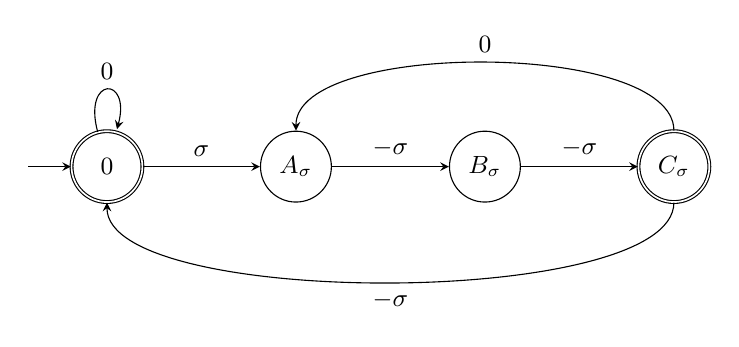
\begin{tikzpicture}[>=stealth, every node/.style={font=\small}]
  \node[draw,circle,double,minimum size=9mm] (z) at (0,0) {$0$};
  \node[draw,circle,minimum size=9mm] (a) at (2.4,0) {$A_\sigma$};
  \node[draw,circle,minimum size=9mm] (b) at (4.8,0) {$B_\sigma$};
  \node[draw,circle,double,minimum size=9mm] (c) at (7.2,0) {$C_\sigma$};
  \draw[->] (-1,0) -- (z);
  \draw[->] (z) edge[loop above] node {$0$} (z);
  \draw[->] (z) -- node[above] {$\sigma$} (a);
  \draw[->] (a) -- node[above] {$-\sigma$} (b);
  \draw[->] (b) -- node[above] {$-\sigma$} (c);
  \draw[->] (c.north) .. controls +(0,1.15) and +(0,1.15) ..
             node[above] {$0$} (a.north);
  \draw[->] (c.south) .. controls +(0,-1.35) and +(0,-1.35) ..
             node[below] {$-\sigma$} (z.south);
 \end{tikzpicture}
\end{document}
